% Color stone chart
\documentclass{article}
\usepackage{geometry}
\geometry{layout=letterpaper,margin=10mm}

\pagestyle{empty}
\usepackage{fontspec,tikz,ifthen,mathptmx}
\usetikzlibrary{calc}
\setmainfont[Ligatures=TeX,Scale=0.80]{Times New Roman}
%\tikzset{font={\fontsize{8pt}{10}\selectfont}}


\begin{document}
\centering
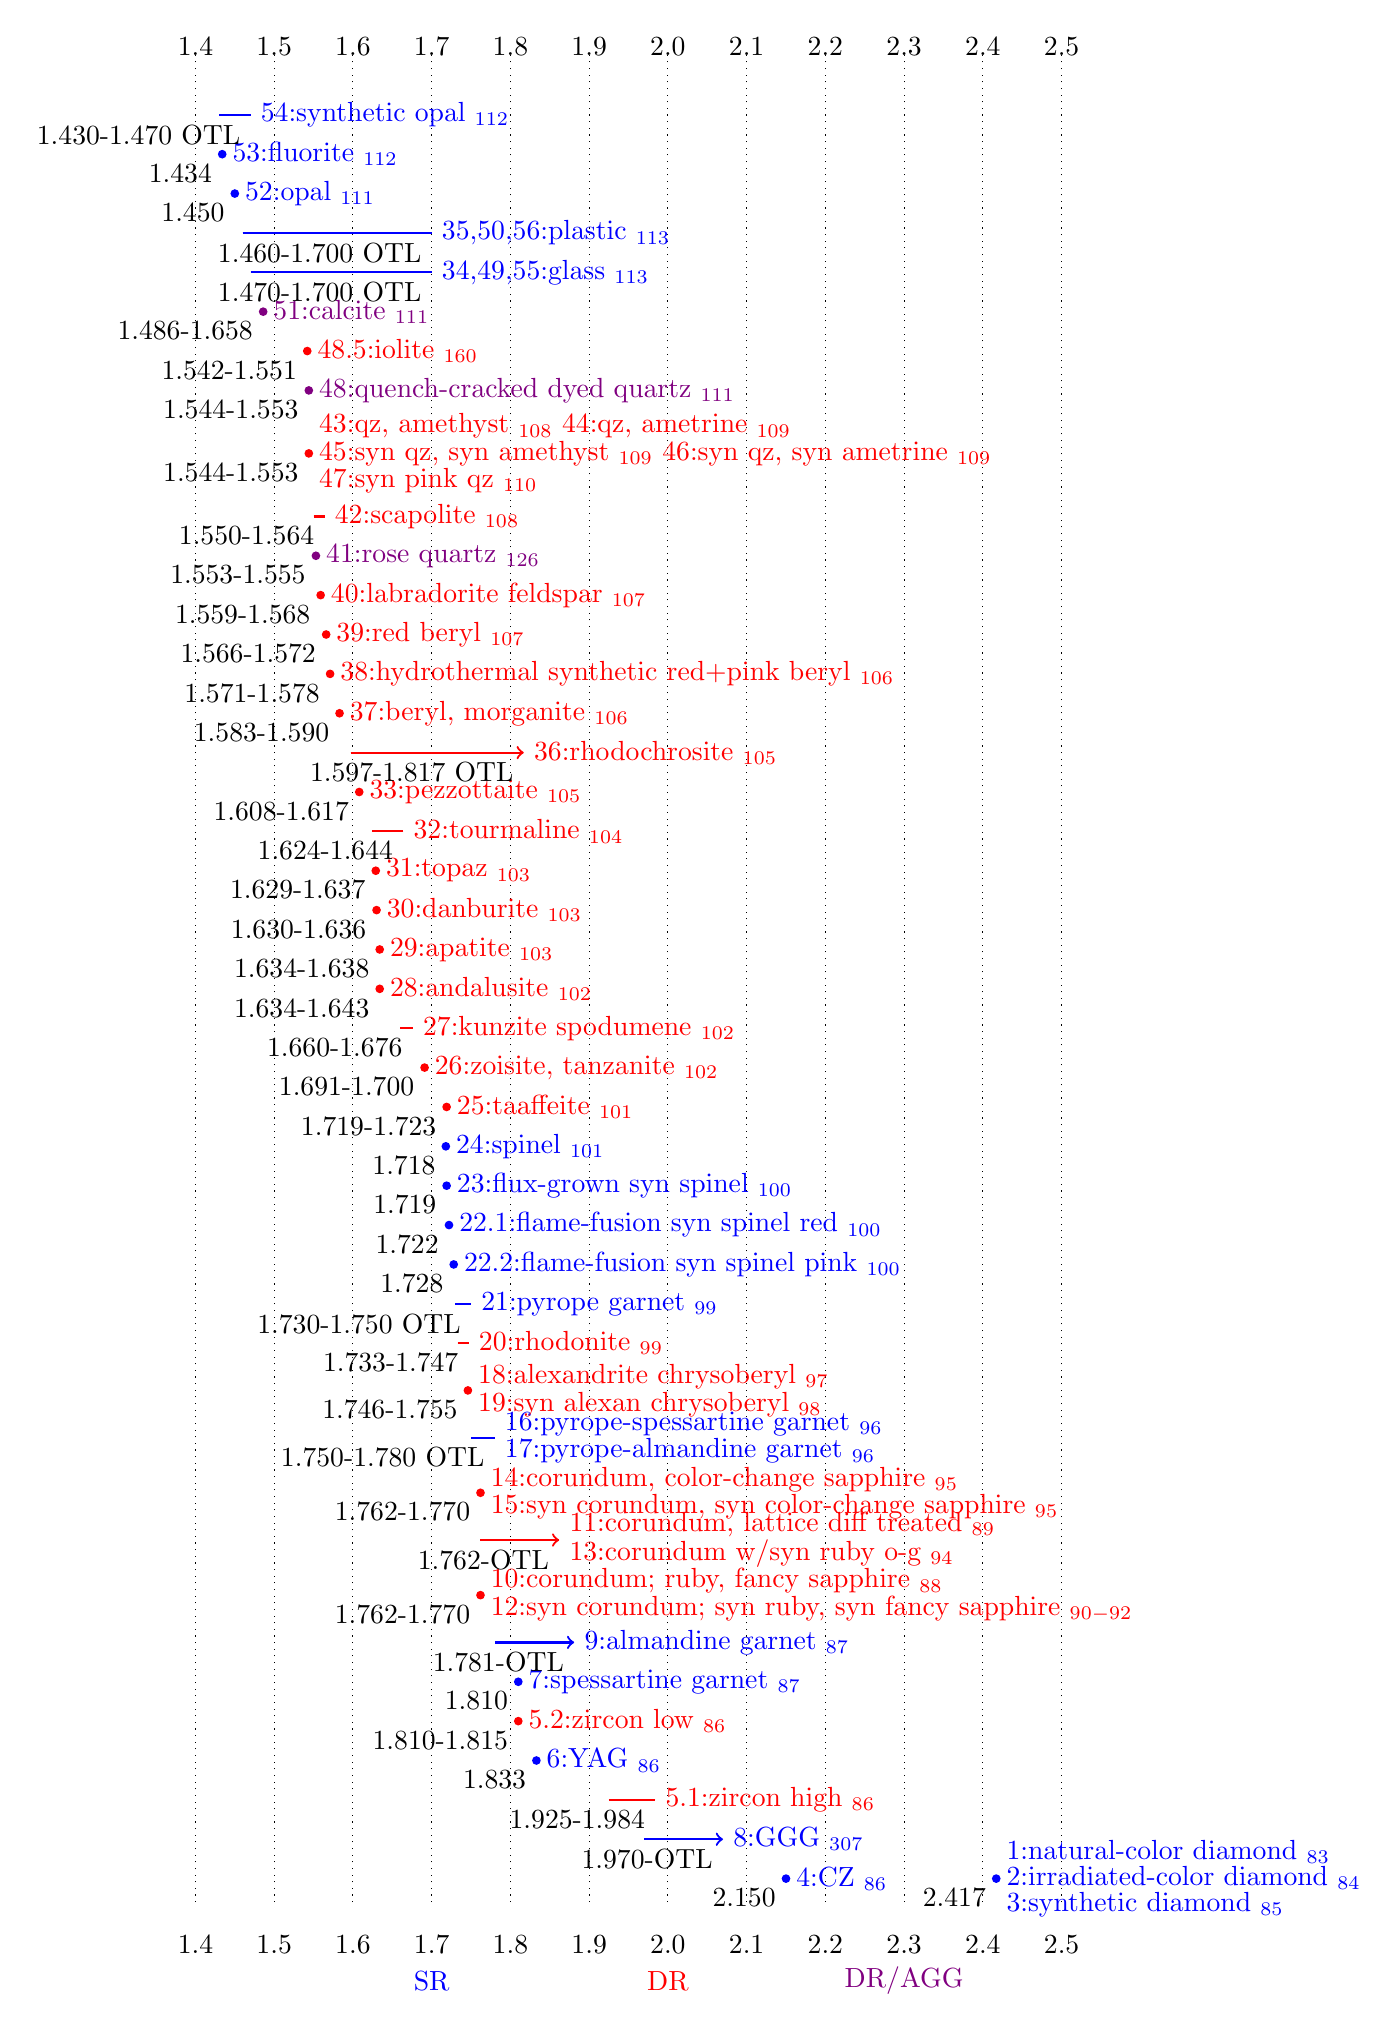
\begin{tikzpicture}[x=1pt,y=1pt,remember picture] % unit must be in pt for convenience of using variables
\tikzset{SR/.style={blue, fill=blue, thick}} 
\tikzset{DR/.style={red, fill=red, thick}} 
\tikzset{DRAGG/.style={violet, fill=violet, thick}} 
\tikzset{vert/.style={black, dotted, thin}} 

\draw[style=SR] (17cm,-10mm) node {SR};
\draw[style=DR] (20cm,-10mm) node {DR};
\draw[style=DRAGG] (23cm,-10mm) node {DR/AGG};
\foreach[evaluate={\xpos=\x*10cm}] \x in {1.4, 1.5, ..., 2.51} {
  % vertical dotted lines
  \draw[style=vert](\xpos, 0mm)--(\xpos, 23.5cm);
  \draw (\xpos,-3mm) node[black, align=center, below] {
    \pgfmathparse{\x}% Evaluate the expression
    \pgfmathprintnumber[    % Print the result
        fixed,
        fixed zerofill,
        precision=1
    ]{\pgfmathresult}%
};
  \draw (\xpos, 238mm) node[black, align=center, below] {
    \pgfmathparse{\x}% Evaluate the expression
    \pgfmathprintnumber[    % Print the result
        fixed,
        fixed zerofill,
        precision=1
    ]{\pgfmathresult}%
};
}
%\draw[style=vert](14cm, 0mm)--(14cm, 10cm);
%\draw[style=vert](15cm, 0mm)--(15cm, 10cm);
%\draw[style=vert](16cm, 0mm)--(16cm, 10cm);
%\draw[style=vert](17cm, 0mm)--(17cm, 10cm);
%\draw[style=vert](18cm, 0mm)--(18cm, 10cm);
%\draw[style=vert](19cm, 0mm)--(19cm, 10cm);
%\draw[style=vert](20cm, 0mm)--(20cm, 10cm);
%\draw[style=vert](21cm, 0mm)--(21cm, 10cm);
%\draw[style=vert](22cm, 0mm)--(22cm, 10cm);
%\draw[style=vert](23cm, 0mm)--(23cm, 10cm);
%\draw[style=vert](24cm, 0mm)--(24cm, 10cm);
%\draw[style=vert](25cm, 0mm)--(25cm, 10cm);
%\draw (24cm,0mm) node[black, align=center, below] {2.4};
%\draw (25cm,0mm) node[black, align=center, below] {2.5};

\edef\curry{3mm}
\filldraw[style=SR] (24.17cm, \curry) circle (0.4mm) node[align=left, right, execute at begin node=\setlength{\baselineskip}{0.8ex}] {1:natural-color diamond ${}_{83}$\\ 2:irradiated-color diamond ${}_{84}$\\ 3:synthetic diamond ${}_{85}$~} node[black, align=left, below left] {2.417};
\filldraw[style=SR] (21.50cm, \curry) circle (0.4mm) node[align=left, right] {4:CZ ${}_{86}$~} node[black, align=left, below left] {2.150};
\pgfmathparse{\curry+5mm}\edef\curry{\pgfmathresult}
\filldraw[style=SR,->] (19.70cm, \curry)--(20.70cm,\curry) node[align=left, right] {8:GGG ${}_{307}$~} node[black, align=left, below left] {1.970-OTL};
\pgfmathparse{\curry+5mm}\edef\curry{\pgfmathresult}
\filldraw[style=DR] (19.25cm, \curry)--(19.84cm,\curry) node[align=left, right] {5.1:zircon high ${}_{86}$~} node[black, align=left, below left] {1.925-1.984};
\pgfmathparse{\curry+5mm}\edef\curry{\pgfmathresult}
\filldraw[style=SR] (18.33cm, \curry) circle (0.4mm) node[align=left, right] {6:YAG ${}_{86}$~} node[black, align=left, below left] {1.833};
\pgfmathparse{\curry+5mm}\edef\curry{\pgfmathresult}
\filldraw[style=DR] (18.10cm, \curry) circle (0.4mm) node[align=left, right] {5.2:zircon low ${}_{86}$~} node[black, align=left, below left] {1.810-1.815};
\pgfmathparse{\curry+5mm}\edef\curry{\pgfmathresult}
\filldraw[style=SR] (18.10cm, \curry) circle (0.4mm) node[align=left, right] {7:spessartine garnet ${}_{87}$~} node[black, align=left, below left] {1.810};
\pgfmathparse{\curry+5mm}\edef\curry{\pgfmathresult}
\filldraw[style=SR,->] (17.81cm, \curry)--(18.81cm,\curry) node[align=left, right] {9:almandine garnet ${}_{87}$~} node[black, align=left, below left] {1.781-OTL};
\pgfmathparse{\curry+6mm}\edef\curry{\pgfmathresult}
\filldraw[style=DR] (17.62cm, \curry) circle (0.4mm) node[align=left, right, execute at begin node=\setlength{\baselineskip}{0.8ex}] {10:corundum; ruby, fancy sapphire ${}_{88}$\\ 12:syn corundum; syn ruby, syn fancy sapphire ${}_{90-92}$~} node[black, align=left, below left] {1.762-1.770};
\pgfmathparse{\curry+7mm}\edef\curry{\pgfmathresult}
\filldraw[style=DR,->] (17.62cm, \curry)--(18.62cm,\curry) node[align=left, right, execute at begin node=\setlength{\baselineskip}{0.8ex}] {11:corundum, lattice diff treated ${}_{89}$\\ 13:corundum w/syn ruby o-g ${}_{94}$~} node[black, align=left, below left] {1.762-OTL};
\pgfmathparse{\curry+6mm}\edef\curry{\pgfmathresult}
\filldraw[style=DR] (17.62cm, \curry) circle (0.4mm) node[align=left, right, execute at begin node=\setlength{\baselineskip}{0.8ex}] {14:corundum, color-change sapphire ${}_{95}$\\ 15:syn corundum, syn color-change sapphire ${}_{95}$~} node[black, align=left, below left] {1.762-1.770};
\pgfmathparse{\curry+7mm}\edef\curry{\pgfmathresult}
\filldraw[style=SR] (17.50cm, \curry)--(17.80cm,\curry) node[align=left, right, execute at begin node=\setlength{\baselineskip}{0.8ex}] {16:pyrope-spessartine garnet ${}_{96}$\\ 17:pyrope-almandine garnet ${}_{96}$~} node[black, align=left, below left] {1.750-1.780 OTL};
\pgfmathparse{\curry+6mm}\edef\curry{\pgfmathresult}
\filldraw[style=DR] (17.46cm, \curry) circle (0.4mm) node[align=left, right, execute at begin node=\setlength{\baselineskip}{0.8ex}] {18:alexandrite chrysoberyl ${}_{97}$\\ 19:syn alexan chrysoberyl ${}_{98}$~} node[black, align=left, below left] {1.746-1.755};
\pgfmathparse{\curry+6mm}\edef\curry{\pgfmathresult}
\filldraw[style=DR] (17.33cm, \curry)--(17.47cm,\curry) node[align=left, right] {20:rhodonite ${}_{99}$~} node[black, align=left, below left] {1.733-1.747};
\pgfmathparse{\curry+5mm}\edef\curry{\pgfmathresult}
\filldraw[style=SR] (17.30cm, \curry)--(17.50cm,\curry) node[align=left, right] {21:pyrope garnet ${}_{99}$~} node[black, align=left, below left] {1.730-1.750 OTL};
\pgfmathparse{\curry+5mm}\edef\curry{\pgfmathresult}
\filldraw[style=SR] (17.28cm, \curry) circle (0.4mm) node[align=left, right] {22.2:flame-fusion syn spinel pink ${}_{100}$~} node[black, align=left, below left] {1.728};
\pgfmathparse{\curry+5mm}\edef\curry{\pgfmathresult}
\filldraw[style=SR] (17.22cm, \curry) circle (0.4mm) node[align=left, right] {22.1:flame-fusion syn spinel red ${}_{100}$~} node[black, align=left, below left] {1.722};
\pgfmathparse{\curry+5mm}\edef\curry{\pgfmathresult}
\filldraw[style=SR] (17.19cm, \curry) circle (0.4mm) node[align=left, right] {23:flux-grown syn spinel ${}_{100}$~} node[black, align=left, below left] {1.719};
\pgfmathparse{\curry+5mm}\edef\curry{\pgfmathresult}
\filldraw[style=SR] (17.18cm, \curry) circle (0.4mm) node[align=left, right] {24:spinel ${}_{101}$~} node[black, align=left, below left] {1.718};
\pgfmathparse{\curry+5mm}\edef\curry{\pgfmathresult}
\filldraw[style=DR] (17.19cm, \curry) circle (0.4mm) node[align=left, right] {25:taaffeite ${}_{101}$~} node[black, align=left, below left] {1.719-1.723};
\pgfmathparse{\curry+5mm}\edef\curry{\pgfmathresult}
\filldraw[style=DR] (16.91cm, \curry) circle (0.4mm) node[align=left, right] {26:zoisite, tanzanite ${}_{102}$~} node[black, align=left, below left] {1.691-1.700};
\pgfmathparse{\curry+5mm}\edef\curry{\pgfmathresult}
\filldraw[style=DR] (16.60cm, \curry)--(16.76cm,\curry) node[align=left, right] {27:kunzite spodumene ${}_{102}$~} node[black, align=left, below left] {1.660-1.676};
\pgfmathparse{\curry+5mm}\edef\curry{\pgfmathresult}
\filldraw[style=DR] (16.34cm, \curry) circle (0.4mm) node[align=left, right] {28:andalusite ${}_{102}$~} node[black, align=left, below left] {1.634-1.643};
\pgfmathparse{\curry+5mm}\edef\curry{\pgfmathresult}
\filldraw[style=DR] (16.34cm, \curry) circle (0.4mm) node[align=left, right] {29:apatite ${}_{103}$~} node[black, align=left, below left] {1.634-1.638};
\pgfmathparse{\curry+5mm}\edef\curry{\pgfmathresult}
\filldraw[style=DR] (16.30cm, \curry) circle (0.4mm) node[align=left, right] {30:danburite ${}_{103}$~} node[black, align=left, below left] {1.630-1.636};
\pgfmathparse{\curry+5mm}\edef\curry{\pgfmathresult}
\filldraw[style=DR] (16.29cm, \curry) circle (0.4mm) node[align=left, right] {31:topaz ${}_{103}$~} node[black, align=left, below left] {1.629-1.637};
\pgfmathparse{\curry+5mm}\edef\curry{\pgfmathresult}
\filldraw[style=DR] (16.24cm, \curry)--(16.64cm,\curry) node[align=left, right] {32:tourmaline ${}_{104}$~} node[black, align=left, below left] {1.624-1.644};
\pgfmathparse{\curry+5mm}\edef\curry{\pgfmathresult}
\filldraw[style=DR] (16.08cm, \curry) circle (0.4mm) node[align=left, right] {33:pezzottaite ${}_{105}$~} node[black, align=left, below left] {1.608-1.617};
\pgfmathparse{\curry+5mm}\edef\curry{\pgfmathresult}
\filldraw[style=DR,->] (15.97cm, \curry)--(18.17cm,\curry) node[align=left, right] {36:rhodochrosite ${}_{105}$~} node[black, align=left, below left] {1.597-1.817 OTL};
\pgfmathparse{\curry+5mm}\edef\curry{\pgfmathresult}
\filldraw[style=DR] (15.83cm, \curry) circle (0.4mm) node[align=left, right] {37:beryl, morganite ${}_{106}$~} node[black, align=left, below left] {1.583-1.590};
\pgfmathparse{\curry+5mm}\edef\curry{\pgfmathresult}
\filldraw[style=DR] (15.71cm, \curry) circle (0.4mm) node[align=left, right] {38:hydrothermal synthetic red+pink beryl ${}_{106}$~} node[black, align=left, below left] {1.571-1.578};
\pgfmathparse{\curry+5mm}\edef\curry{\pgfmathresult}
\filldraw[style=DR] (15.66cm, \curry) circle (0.4mm) node[align=left, right] {39:red beryl ${}_{107}$~} node[black, align=left, below left] {1.566-1.572};
\pgfmathparse{\curry+5mm}\edef\curry{\pgfmathresult}
\filldraw[style=DR] (15.59cm, \curry) circle (0.4mm) node[align=left, right] {40:labradorite feldspar ${}_{107}$~} node[black, align=left, below left] {1.559-1.568};
\pgfmathparse{\curry+5mm}\edef\curry{\pgfmathresult}
\filldraw[style=DRAGG] (15.53cm, \curry) circle (0.4mm) node[align=left, right] {41:rose quartz ${}_{126}$~} node[black, align=left, below left] {1.553-1.555};
\pgfmathparse{\curry+5mm}\edef\curry{\pgfmathresult}
\filldraw[style=DR] (15.50cm, \curry)--(15.64cm,\curry) node[align=left, right] {42:scapolite ${}_{108}$~} node[black, align=left, below left] {1.550-1.564};
\pgfmathparse{\curry+8mm}\edef\curry{\pgfmathresult}
\filldraw[style=DR] (15.44cm, \curry) circle (0.4mm) node[align=left, right, execute at begin node=\setlength{\baselineskip}{0.8ex}] {43:qz, amethyst ${}_{108}$ 44:qz, ametrine ${}_{109}$\\ 45:syn qz, syn amethyst ${}_{109}$ 46:syn qz, syn ametrine ${}_{109}$\\ 47:syn pink qz ${}_{110}$~} node[black, align=left, below left] {1.544-1.553};
\pgfmathparse{\curry+8mm}\edef\curry{\pgfmathresult}
\filldraw[style=DRAGG] (15.44cm, \curry) circle (0.4mm) node[align=left, right] {48:quench-cracked dyed quartz ${}_{111}$~} node[black, align=left, below left] {1.544-1.553};
\pgfmathparse{\curry+5mm}\edef\curry{\pgfmathresult}
\filldraw[style=DR] (15.42cm, \curry) circle (0.4mm) node[align=left, right] {48.5:iolite ${}_{160}$~} node[black, align=left, below left] {1.542-1.551};
\pgfmathparse{\curry+5mm}\edef\curry{\pgfmathresult}
\filldraw[style=DRAGG] (14.86cm, \curry) circle (0.4mm) node[align=left, right] {51:calcite ${}_{111}$~} node[black, align=left, below left] {1.486-1.658};
\pgfmathparse{\curry+5mm}\edef\curry{\pgfmathresult}
\filldraw[style=SR] (14.70cm, \curry)--(17.00cm,\curry) node[align=left, right] {34,49,55:glass ${}_{113}$~} node[black, align=left, below left] {1.470-1.700 OTL};
\pgfmathparse{\curry+5mm}\edef\curry{\pgfmathresult}
\filldraw[style=SR] (14.60cm, \curry)--(17.00cm,\curry) node[align=left, right] {35,50,56:plastic ${}_{113}$~} node[black, align=left, below left] {1.460-1.700 OTL};
\pgfmathparse{\curry+5mm}\edef\curry{\pgfmathresult}
\filldraw[style=SR] (14.50cm, \curry) circle (0.4mm) node[align=left, right] {52:opal ${}_{111}$~} node[black, align=left, below left] {1.450};
\pgfmathparse{\curry+5mm}\edef\curry{\pgfmathresult}
\filldraw[style=SR] (14.34cm, \curry) circle (0.4mm) node[align=left, right] {53:fluorite ${}_{112}$~} node[black, align=left, below left] {1.434};
\pgfmathparse{\curry+5mm}\edef\curry{\pgfmathresult}
\filldraw[style=SR] (14.30cm, \curry)--(14.70cm,\curry) node[align=left, right] {54:synthetic opal ${}_{112}$~} node[black, align=left, below left] {1.430-1.470 OTL};
\end{tikzpicture}
\end{document}
